\begin{figure*}[h]
    \centering
    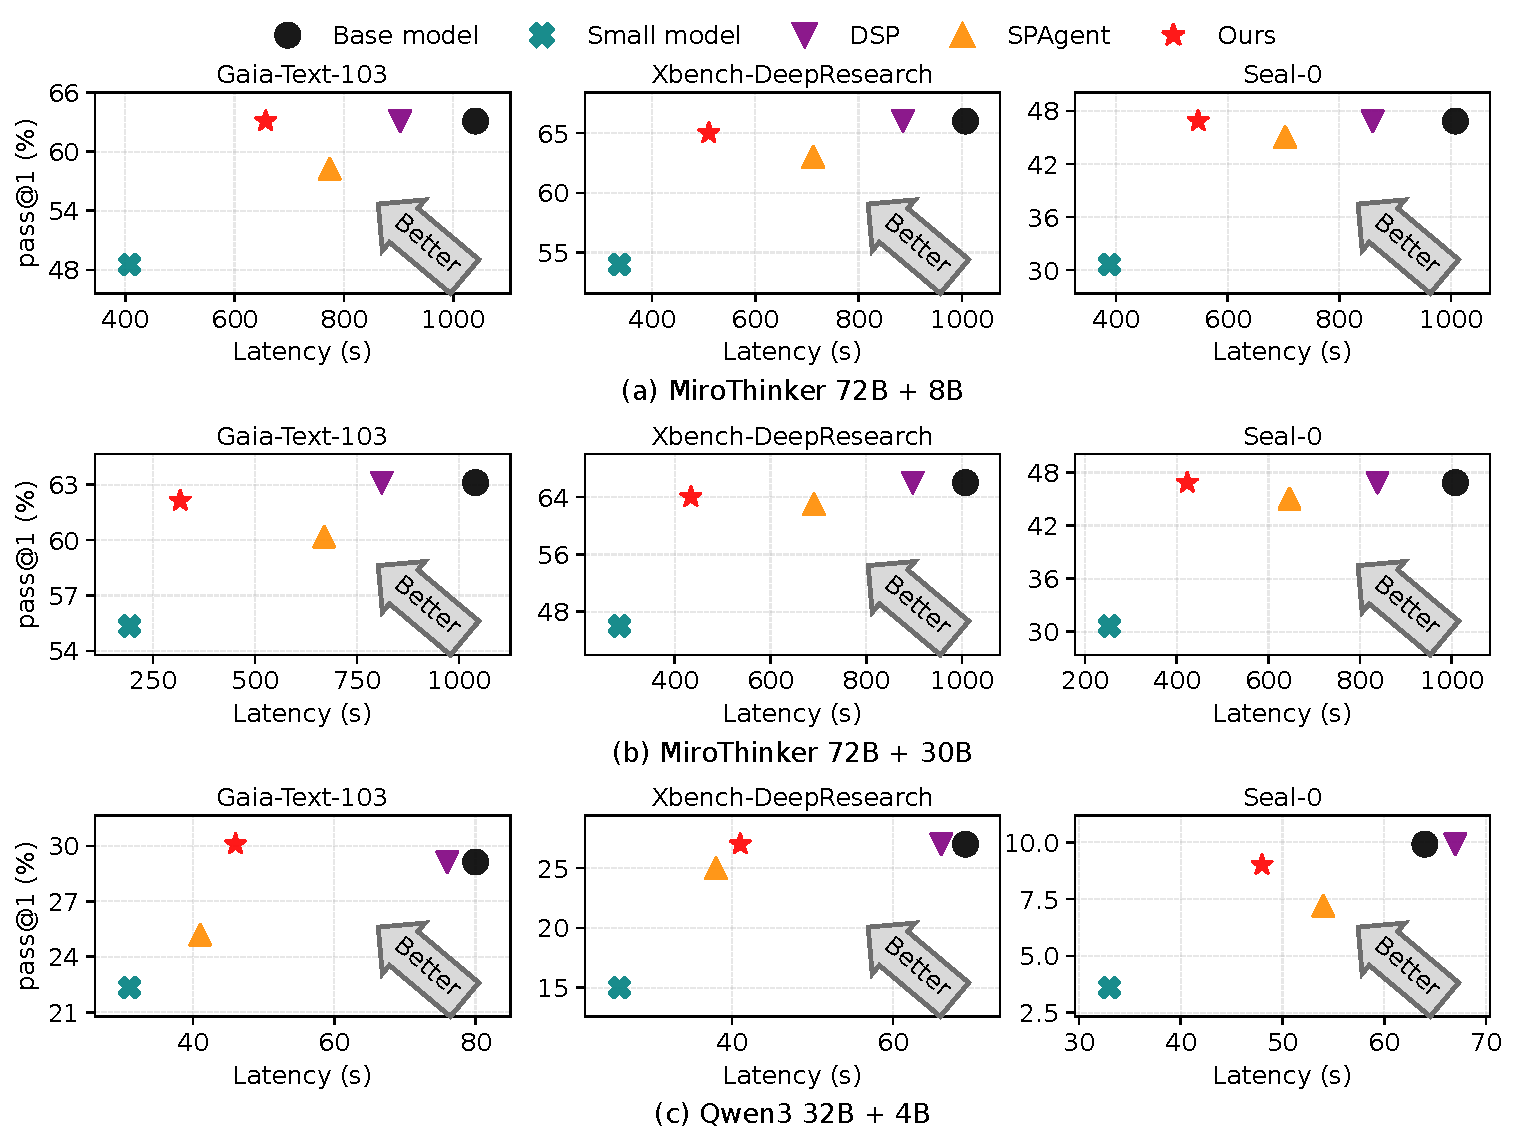
\includegraphics[width=0.9\linewidth]{figs/main_exp_results.pdf}
    \caption{Comparison of the accuracy (pass@1) and latency of different schemes across model combinations.
\method{} consistently reduces end-to-end latency by \textbf{1.33–3.28$\times$} (\(\sim\)2$\times$ on average) over the base model while maintaining comparable accuracy.
Compared with DSP and SPAgent, \method{} achieves a better accuracy–latency trade-off across all datasets and model pairs.}
    \label{fig:main_results}
\end{figure*}

\section{Experiments}

\subsection{Experimental Setup}

\paragraph{Models.}
We evaluate \method{} under three dual-model configurations: 
MiroThinker-v1.0-72B + MiroThinker-v1.0-8B, 
MiroThinker-v1.0-72B + MiroThinker-v1.0-30B-A3B, and 
Qwen3-32B + Qwen3-4B~\cite{team2025mirothinker,yang2025qwen3}. All models are deployed single-tenant with one \textsc{NVIDIA} A100 GPU per model and batch\_size=$4$ for inference. The MiroThinker Models were quantized to 4-bit for inference, while the Qwen Models use native FP8 quantization, to avoid out-of-memory in GPUs.

\paragraph{Datasets.}
Experiments are conducted on three representative deep-research benchmarks:
including GAIA-Text-103~\cite{wu2025webdancer}, XBench-DeepSearch~\cite{chen2025xbench} and Seal-0~\cite{pham2025sealqa}.

\paragraph{Frameworks.}

We build our agent on the MiroMind deep‑research framework.
Tool invocation follows the MCP (Model Context Protocol) interface to standardize tool signatures and I/O, ensuring consistent argument formatting and result parsing across models and datasets.
Within this setup, Search calls are executed via the Bing API, and Visit operations (page fetching and readable content extraction) are served by Jina, providing a fixed backend for web querying and page processing throughout all experiments. The models are serving under SGLang\cite{zheng2024sglang}.

\paragraph{Baselines.}

We compare with two speculative agent frameworks: DSP~\cite{guan2025dynamic} and SPAgent~\cite{huang2025reducing}.
DSP targets planning tasks and accepts a draft only if it matches the base action (minimum edit distance),
while SPAgent is tailored to web search, skipping verification early and enforcing strict action matching later.
In contrast to their uniform drafting and action-alignment verification, \method{} uses heterogeneous drafting for System~2/System~1 actions and semantic verification that accepts trajectory-consistent drafts without exact action equivalence.

\paragraph{Verifier threshold.}
We tune the verifier threshold $\tau$ on a held-out split of GAIA, targeting an intervention rate of $\sim$20\%,
and reuse the same $\tau$ in our experiments.

\subsection{Main Results}

Figure~\ref{fig:main_results} reports end-to-end \emph{latency} vs.\ \emph{pass@1} across three model pairs and three deep‑research benchmarks. 
Overall, \method{} attains \textbf{1.33–3.28$\times$} speedup over the base model, averaging \textbf{$\sim$2$\times$}, while maintaining comparable pass@1.
Across datasets and model combinations, the points for \method{} consistently move left (lower latency) with negligible accuracy degradation, indicating a better accuracy–latency operating point than uniform speculative baselines.

By analyzing each model pair, we observe 1.8$\times$ acceleration on MiroThinker‑72B + 8B, 2.6$\times$ on MiroThinker‑72B + 30B, and 1.5$\times$ on Qwen3‑32B + 4B.
The larger gain with the 30B configuration arises from its MoE design that each forward activates roughly \emph{3B} parameters; at the same time, its stronger base capability reduces the number of base model interventions, further reducing end‑to‑end time.
Consequently, using 30B‑A3B as the base model delivers the highest overall speedup among the evaluated pairs.


\subsection{Ablation Studies}

\subsubsection{speculation methods}

\begin{table}[h]
  \centering
  \caption{Performance under different speculation schemes.}
  \label{tab:spec_ablation}
  \setlength{\tabcolsep}{4pt}
  \begin{tabular}{ccccc}
    \toprule
    \textbf{Models} & \textbf{Datasets} & \textbf{Speculation} & \textbf{Acc} & \textbf{Lat} \\
    \midrule
    \multirow{8}{*}{\makecell[c]{Miro\\72B+8B}} 
      & \multirow{4}{*}{GAIA}
        & Origin         & 63.1 & 1041 \\
      & & LLM w/o Reason & 59.2 & 575 \\
      & & SLM w/ Reason  & 56.3 & 651 \\
      & & Heterogeneous   & 63.1 & 605 \\
      \cmidrule(lr){2-5}
      & \multirow{4}{*}{Xbench}
        & Origin         & 66    & 1007 \\
      & & LLM w/o Reason & 65    & 492 \\
      & & SLM w/ Reason  & 65    & 501 \\
      & & Heterogeneous   & 66    & 480 \\
    \midrule
    \multirow{8}{*}{\makecell[c]{Qwen\\32B+4B}} 
      & \multirow{4}{*}{GAIA}
        & Origin         & 29.1 & 80 \\
      & & LLM w/o Reason & 27.1  & 67 \\
      & & SLM w/ Reason  & 25.2  & 32 \\
      & & Heterogeneous   & 30.1 & 46 \\
      \cmidrule(lr){2-5}
      & \multirow{4}{*}{Xbench}
        & Origin         & 27    & 69 \\
      & & LLM w/o Reason & 25    & 46 \\
      & & SLM w/ Reason  & 26    & 49 \\
      & & Heterogeneous   & 27    & 41 \\
    \bottomrule
  \end{tabular}
\end{table}

To analyze the impact of heterogeneous speculation on performance, we fix the verification setting and vary only the speculation strategy, comparing our heterogeneous approach against the small-model-only methods and skipping-reasoning methods.
As shown in Table~\ref{tab:spec_ablation}, heterogeneous speculation consistently achieves a better accuracy–latency balance than either \textit{LLM w/o Reason} or \textit{SLM w/ Reason}, maintaining accuracy while reducing end-to-end latency across model pairs and datasets.

\subsubsection{Intervention Rate}

\begin{figure}
    \centering
    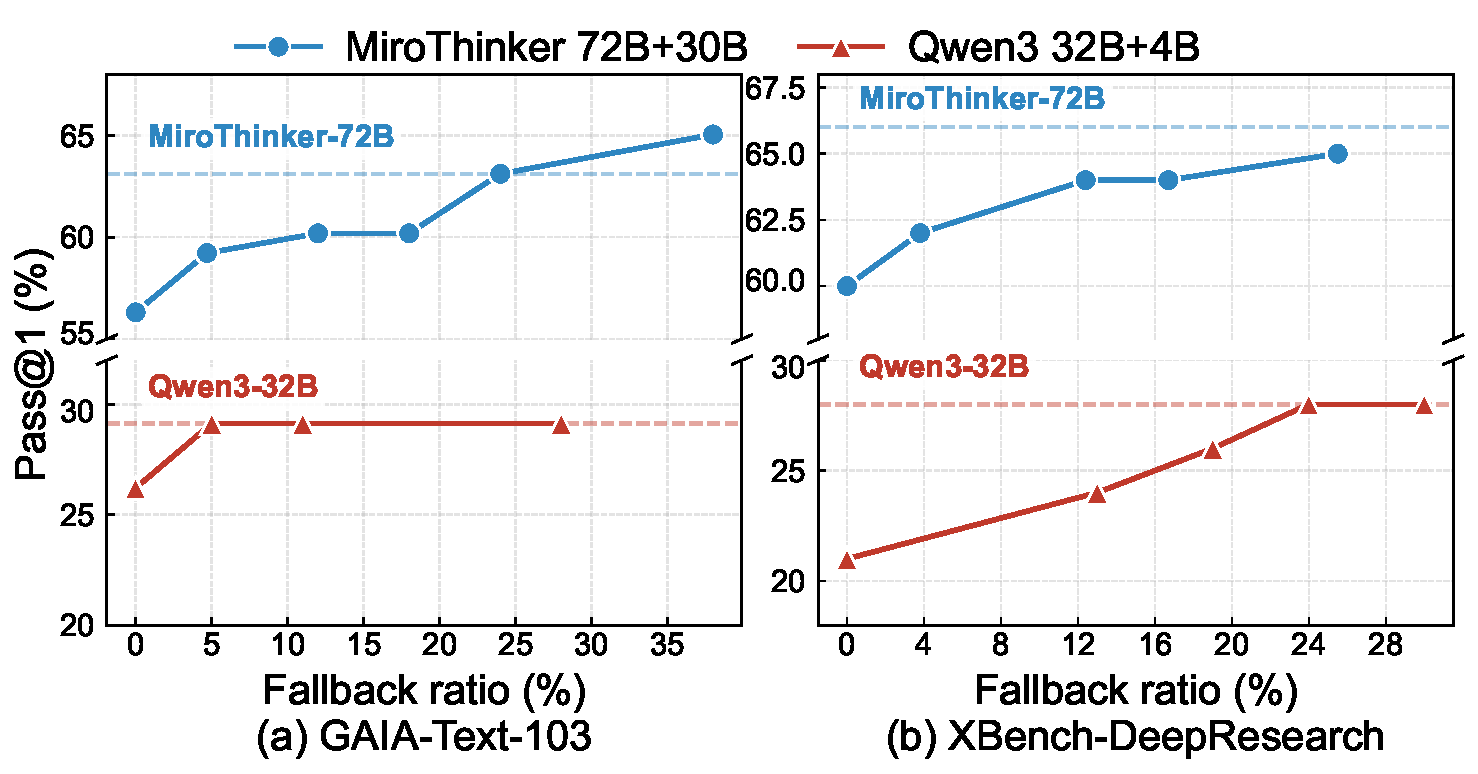
\includegraphics[width=\linewidth]{figs/threshold.pdf}
    \caption{Accuracy (pass@1) as a function of the reasoning intervention rate under a fixed drafting policy.}
    \label{fig:fallback_ratio}
\end{figure}

We study how accuracy changes with the frequency of the large model intervention. With a fixed speculator, we vary the verifier threshold, which indirectly controls the intervention rate. Accuracy increases as the intervention rate rises and then saturates. In practice, we observe that an intervention rate of about \textbf{20\% to 30\%} already reaches accuracy comparable to the base model, while retaining most of the latency benefit of heterogeneous speculation.

This trend is consistent across model families and datasets, with minor shifts in the saturation point. While tighter thresholds further improve accuracy, the returns diminish once the rate reaches the low-to-mid twenties. We therefore tune the threshold to target an intervention rate near 20\%, recovering near-base accuracy without sacrificing the efficiency benefits of sparse large-model reasoning.
